The Parameter Object is a design pattern utilized to group logically related method parameters into a separate entity,
typically a data class or structure.
Subsequently, the method is refactored to accept a single parameter object rather than multiple parameters.
This Parameter Object is typically immutable and contains only accessor methods.
The Parameter Object was introduced in the book Refactoring: Improving the Design of Existing Code by Martin Fowler
as one of the refactoring techniques~\cite[Chapter~10]{fowler1999refactoring}.

Figure~\ref{fig:group_single_entity} illustrates the extraction of three parameters, namely \textit{igmpType},
\textit{maxResponseTime}, and \textit{groupAddress}, into a new class named \textit{IgmpPacket}.
The \textit{IgmpPacketWriter} service is then refactored to accept two parameters instead of five in the method
\textit{writeIgmpPacket}: \textit{igmpPacket} and \textit{outputStream}.
Additionally, the \textit{IgmpPacket} class includes Factory methods for the straightforward creation of various types
of IGMP packets, responsible for filling in correct constant values for each type.
More information about the Factory design pattern can be found in~\cite[Chapter~20]{posa4}.

\begin{figure}[!htb]
    \centering
    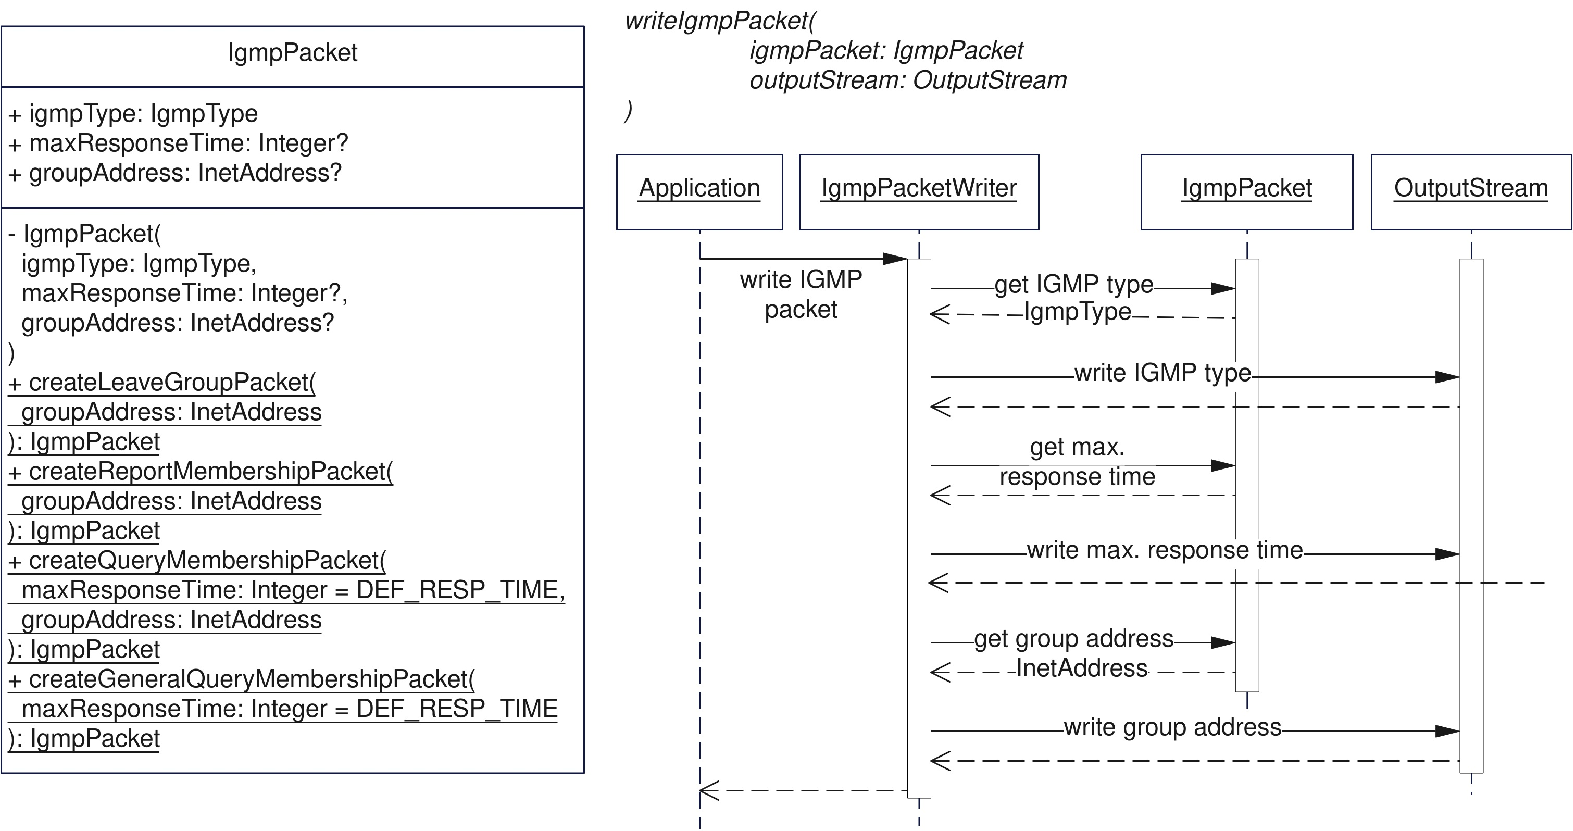
\includegraphics[width=1.0
    \textwidth]{group_single_entity}
    \caption{Parameter Objects: Extraction of a group of parameters into a separate class}
    \label{fig:group_single_entity}
\end{figure}

Instead of utilizing Factory methods, the Builder pattern can be employed to create instances
of the \textit{IgmpPacket} class, especially when there are many optional parameters that clients can set
~\cite[Chapter~20]{posa4}.
Figure~\ref{fig:group_build_single_entity} demonstrates how the Builder pattern can be used in creating
an instance of the \textit{IgmpPacket} class.
The entire building process occurs in the \textit{build} method, invoked by the client after setting
all necessary parameters.
This method often encompasses logic related to parameter validation, default value assignment, or value transformation.

\begin{figure}[!htb]
    \centering
    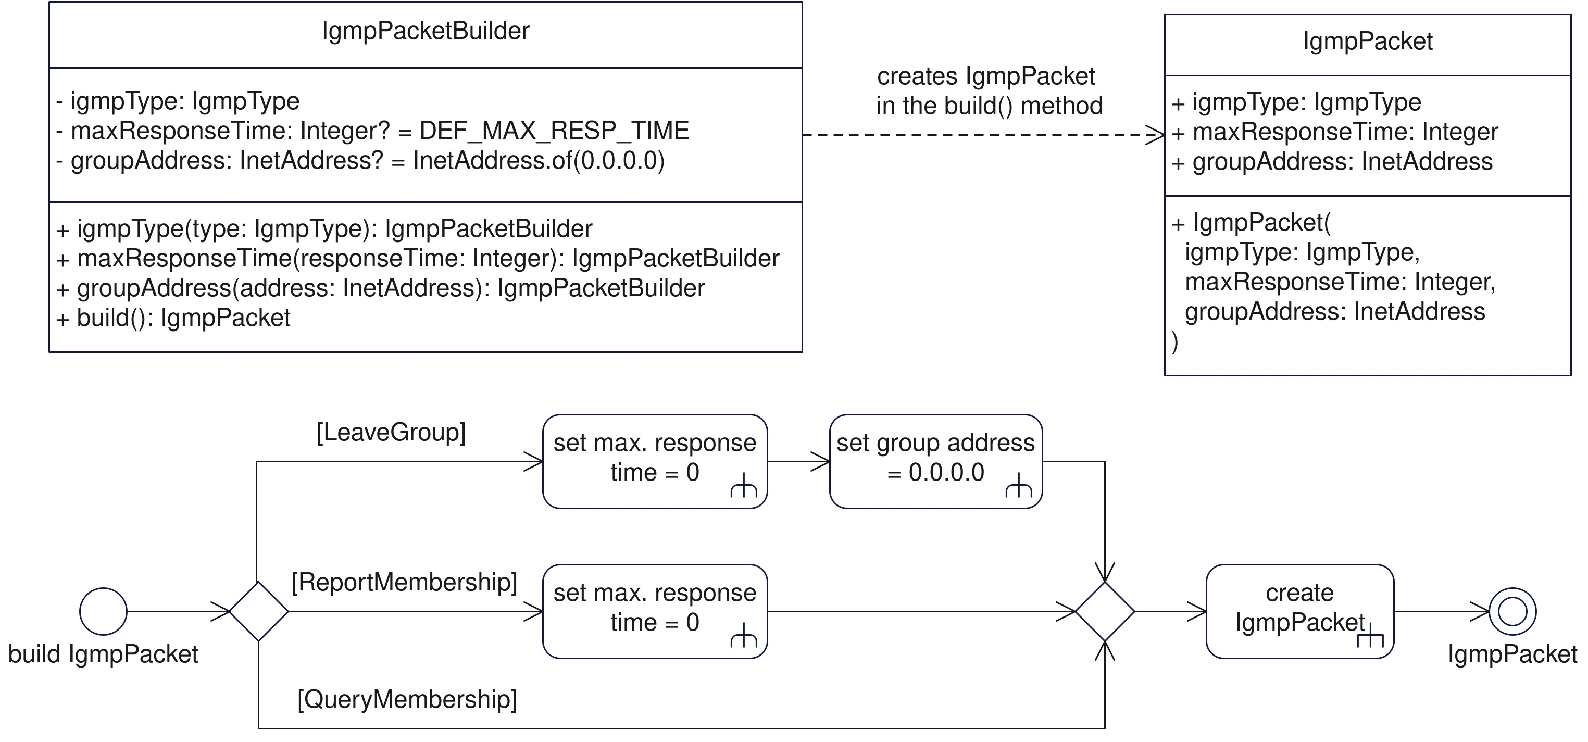
\includegraphics[width=1.0
    \textwidth]{group_build_single_entity}
    \caption{Parameter Objects: Using Builder pattern to create IgmpPacket object}
    \label{fig:group_build_single_entity}
\end{figure}

Figure~\ref{fig:group_build_structure} displays the next iteration of the Builder design pattern.
In this case, the builder class creates specific instances of \textit{IgmpPacket} subtypes -
\textit{IgmpLeaveGroupPacket}, \textit{IgmpReportMembershipPacket}, or \textit{IgmpQueryMembershipPacket}.
Defining multiple subtypes of the \textit{IgmpPacket} class is a superior approach if there are structural differences
between IGMP packet types or when specific behavior needs to be associated with a particular type.

\begin{figure}[!htb]
    \centering
    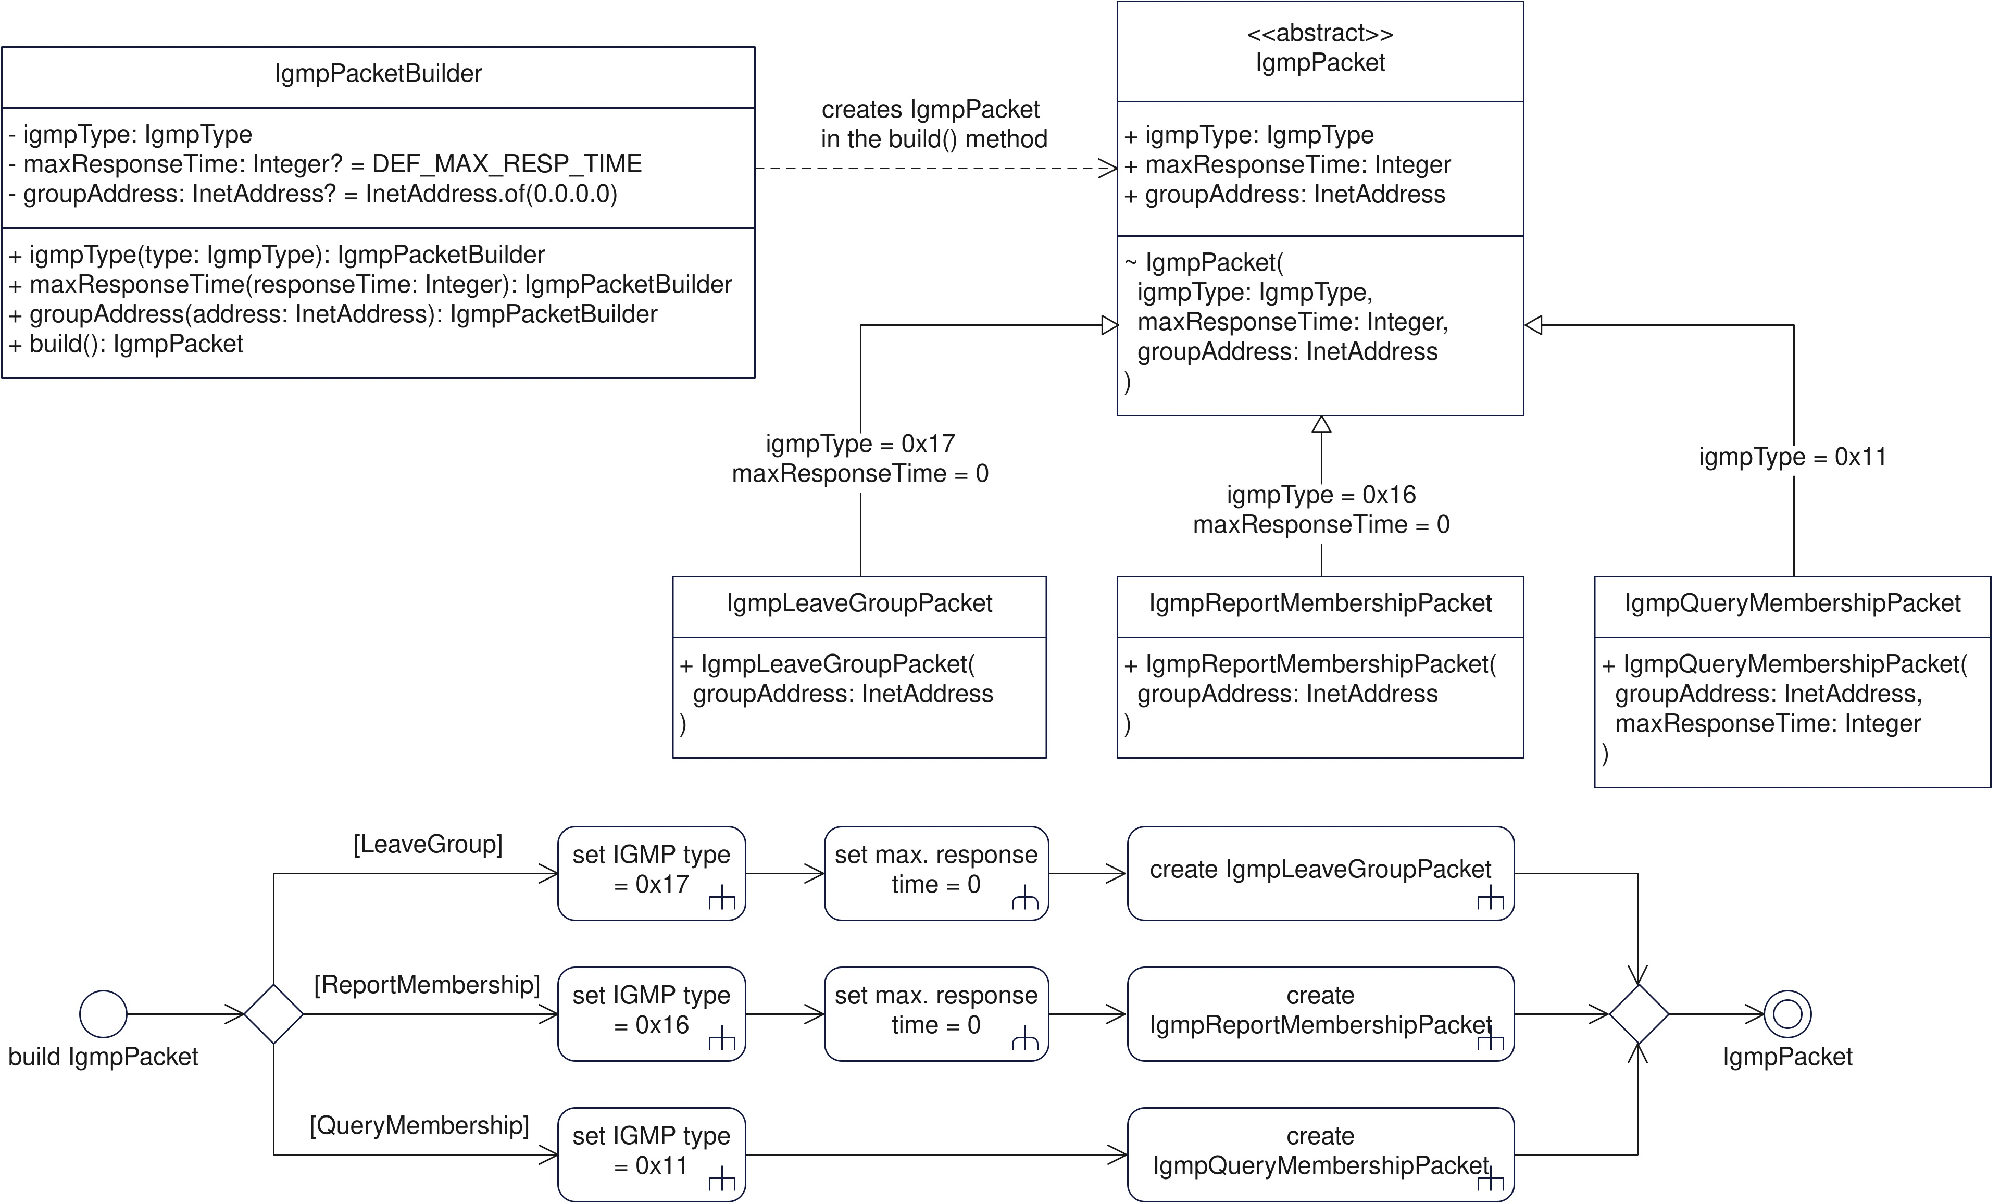
\includegraphics[width=1.0
    \textwidth]{group_build_structure}
    \caption{Parameter Object: Using Builder pattern to create object of IgmpPacket subtype}
    \label{fig:group_build_structure}
\end{figure}

At times, it is advantageous to shift the responsibility for writing IGMP packets to the output stream
from \textit{IgmpPacketWriter} to \textit{IgmpPacket} itself, as illustrated
in Figure~\ref{fig:group_write_from_igmp_packet}.
While this approach enables the use of polymorphism to invoke the correct method for writing IGMP packets,
it introduces tight coupling between \textit{IgmpPacket} and \textit{OutputStream} with serialization business logic,
potentially leading to issues in dependency management and code maintainability.

\begin{figure}[!htb]
    \centering
    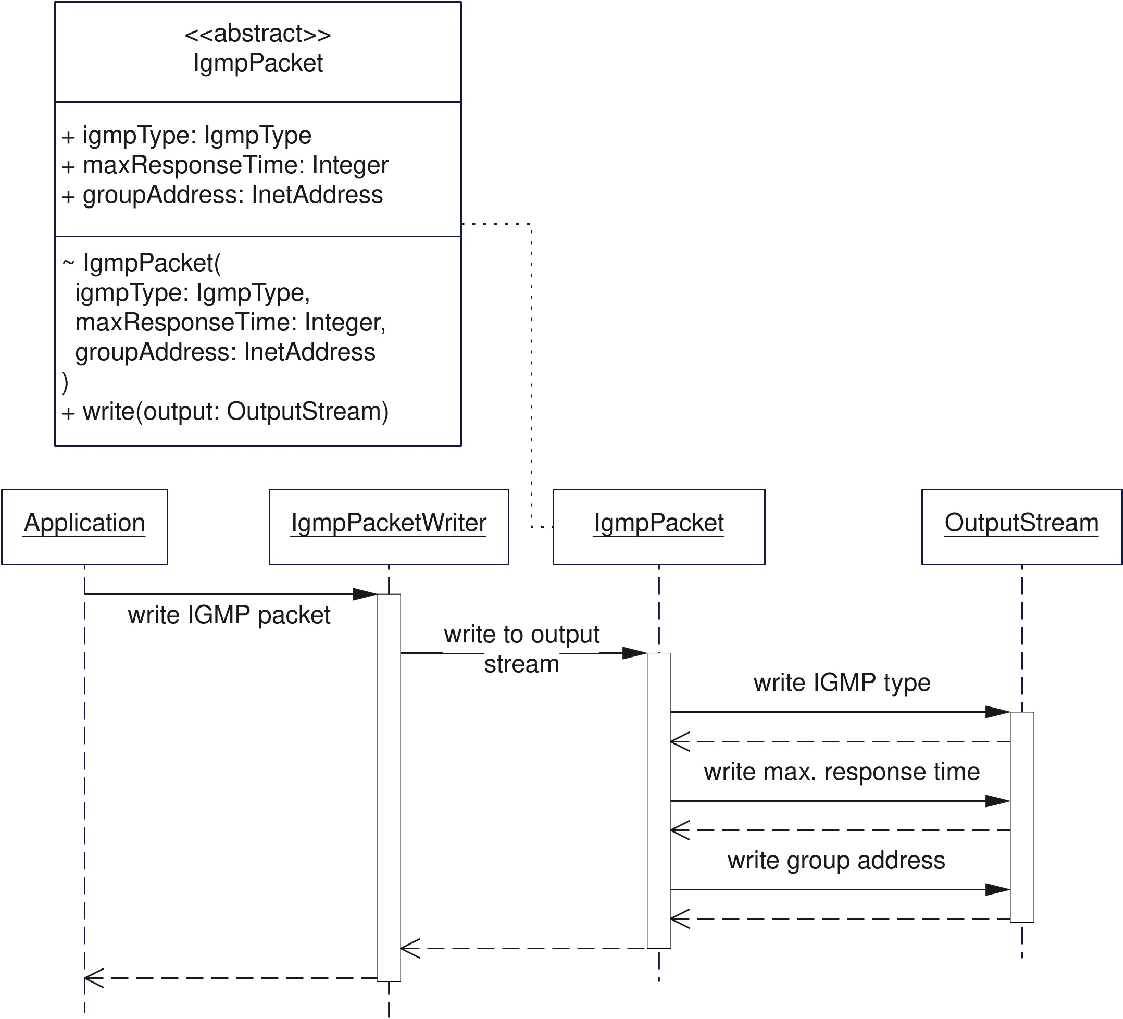
\includegraphics[width=0.8
    \textwidth]{group_write_from_igmp_packet}
    \caption{Parameter Object: Moving write responsibility from IgmpPacketWriter to IgmpPacket}
    \label{fig:group_write_from_igmp_packet}
\end{figure}

The final variation of the Parameter Object approach is depicted in Figure~\ref{fig:group_visitor},
incorporating the Visitor design pattern.
In this scenario, the \textit{IgmpPacket} class accepts \textit{IgmpPacketProcessor} as a parameter
in the method \textit{process}.
\textit{IgmpPacketProcessor} represents the interface, and \textit{IgmpPacketWriter} implements this interface
with one method implementation for each subtype of \textit{IgmpPacket}.
The advantage lies in introducing an abstraction layer, the generic visitor interface \textit{IgmpPacketProcessor},
between \textit{IgmpPacket} and \textit{IgmpPacketWriter} - interface is not directly coupled with implementation.
However, the drawback is the presence of a double-dispatching mechanism, adding complexity to the implementation.
Visitor design pattern is described in more detail in~\cite[Chapter~18]{posa4}.

\begin{figure}[!htb]
    \centering
    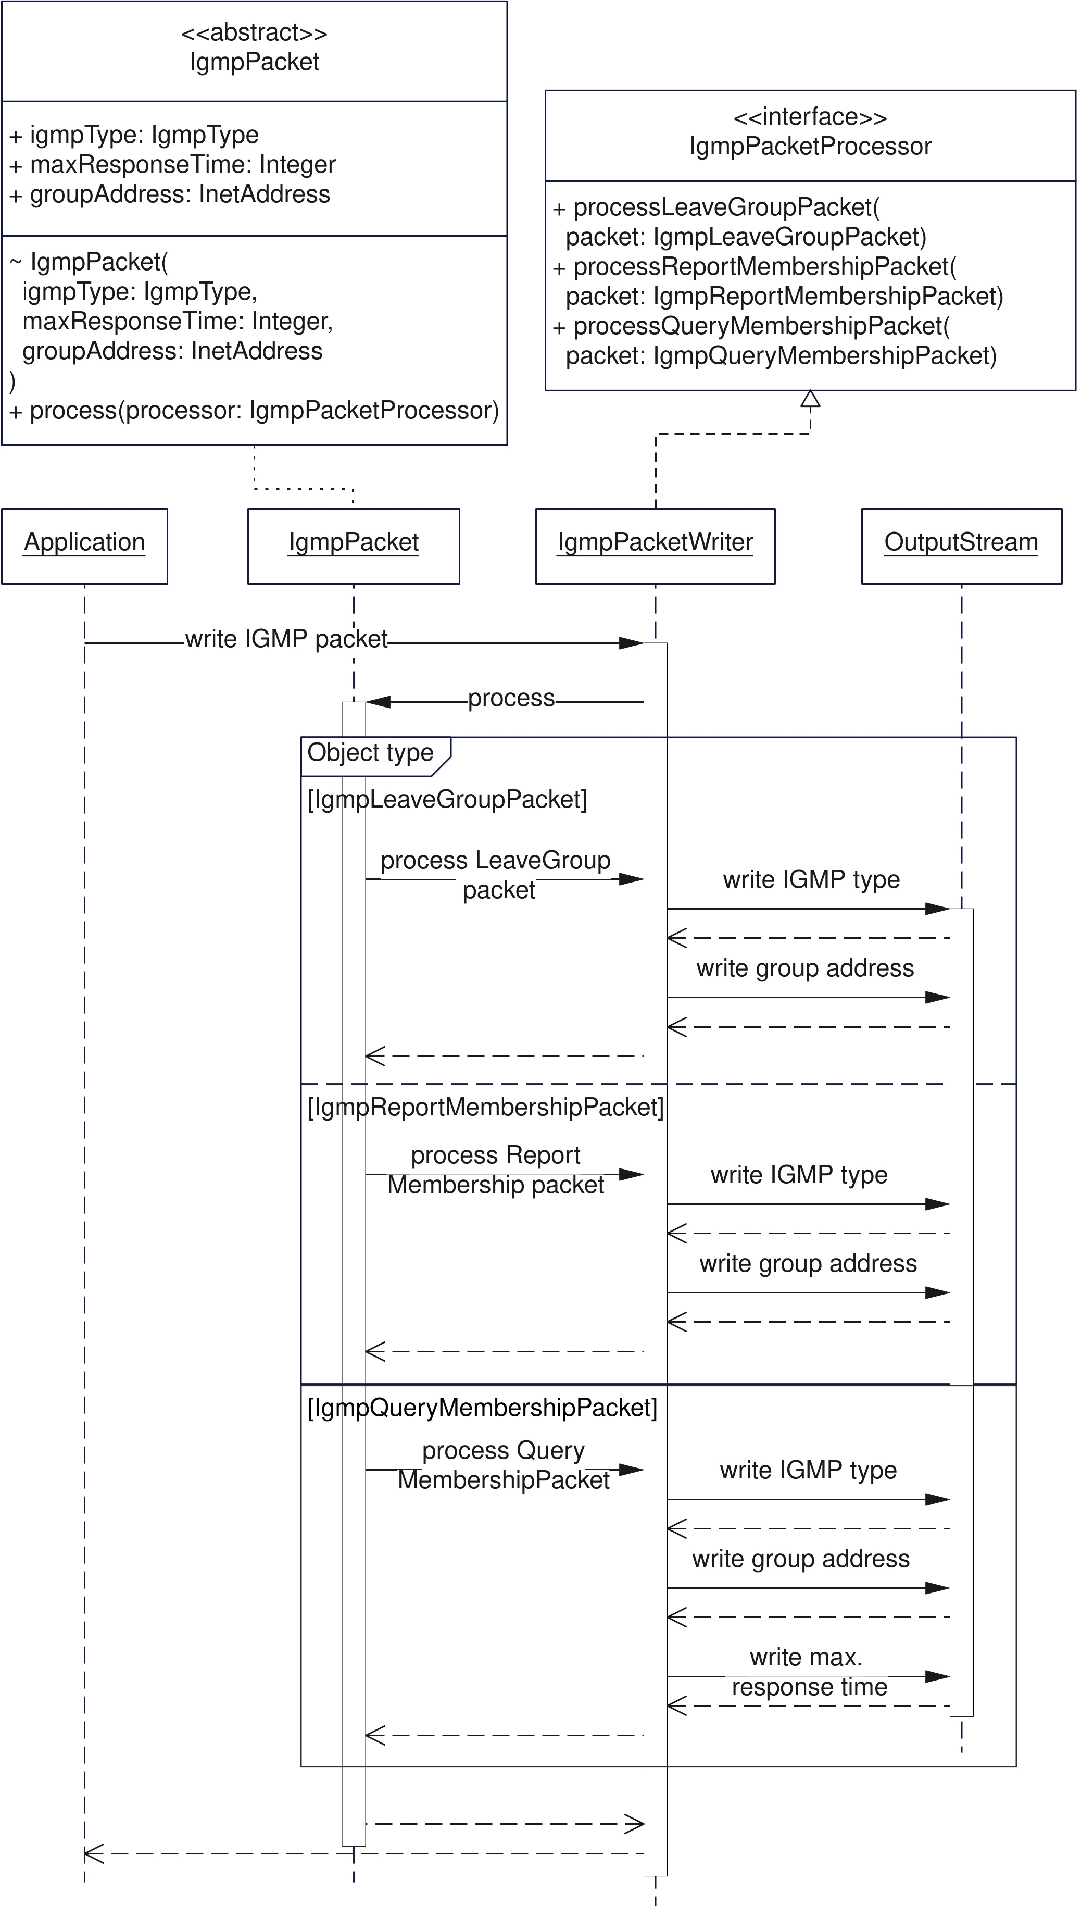
\includegraphics[width=0.75
    \textwidth]{group_visitor}
    \caption{Parameter Objects: Using Visitor design pattern to invoke actions on IgmpPacket subtype}
    \label{fig:group_visitor}
\end{figure}

Benefits of the Parameter Object design pattern:

\begin{itemize}
    \item Enhanced code readability:
    Grouping closely related parameters into a single entity significantly improves the readability of the code.
    This organizational approach makes it easier to understand the purpose and context of the parameters.
    Additionally, the use of multiple Parameter Objects in the same method is possible, enhancing code structure.
    \item Reusability across interfaces:
    Parameter Objects can be effectively reused across multiple interface methods and their
    corresponding implementations.
    This reusability fosters consistency and reduces redundancy in code.
    \item API robustness:
    Constructing Parameter Objects using the Builder or Factory pattern, rather than directly calling the constructor
    of the created class, makes the API less fragile.
    This ensures a more robust and adaptable architecture.
\end{itemize}

Drawbacks of the Parameter Object design pattern:

\begin{itemize}
    \item Encapsulation risks:
    If a Parameter Object is mutable, there is a risk of encapsulation violation.
    Modifications to the object's state could lead to unintended side effects,
    impacting the stability and reliability of the code.
    \item Overuse concerns:
    Excessive use of Parameter Objects may lead to the creation of an abundance of classes, potentially complicating
    the codebase.
    Careful consideration should be given to whether each parameter grouping truly warrants a distinct object.
    \item Exposure of implementation details:
    Utilizing this design pattern raises the risk of exposing implementation details through the API\@,
    if Parameter Object contains some business logic.
    Developers need to exercise caution to maintain a clear separation between the public API and internal
    implementation specifics.
\end{itemize}

Common use-cases of the Parameter Object design pattern:

\begin{itemize}
    \item Parameter compression:
    When dealing with a long list of parameters, the Parameter Object pattern is useful for compressing them into
    a single or just a few Parameter Objects.
    This simplifies method signatures and enhances code conciseness.
    \item Grouping optional parameters:
    Parameter Objects are effective in grouping optional parameters, eliminating the need for method overloading
    and avoiding the presence of nullable parameters.
    This results in cleaner and more maintainable code.
    \item Consistency assurance:
    By grouping repetitive lists of parameters into Parameter Objects, the design pattern helps ensure consistency
    across method definitions.
    This reduces the likelihood of errors and promotes a standardized approach to parameter handling.
\end{itemize}
